\chapter{Valid Outcomes of Positive Support Size Four}

\section{Hyperfield Criterion}

We introduce the \emph{Hyperfield Criterion}. This criterion can be interpreted as constraints on the support of valid outcomes.

\begin{definition}
    Let \( H \coloneqq \left\{ -1, 0, 1 \right\} \). We define the addition \( + : H \times H \to 2^H \setminus \left\{ \emptyset \right\} \) on \( H \) as follows: \( 0 + x = \left\{ x \right\},  1 + 1 = \left\{ 1 \right\},1 + (-1) = H \), and \( (-1) + (-1) = \left\{ -1 \right\} \) for all \( x \in H \).
    Multiplication \( \times : H \times H \to H \) is defined as usual. We call \( H \) the \emph{sign hyperfield}.
\end{definition}

For singleton sets \( \{ x \} \), we often write \( x \) instead of \( \{ x \} \); thus, \( 1 + 1 = 1 \) and \( (-1) + 0 = -1 \).

\begin{remark}
    The tuple \( (H, + , \cdot, 0, 1) \) is called a \emph{hyperfield}. For more details, see \cite{baker2018matroids}. In summary, a hyperfield satisfies the following properties:
    \begin{enumerate}
        \item  The maps \( + \) and \( \cdot \) are symmetric;
        \item \( (H \setminus \left\{ 0 \right\}, \cdot, 1) \) is a group;
        \item \( 0 \cdot x = 0 \) and \( 0 + x = x \) hold for all \( x \in H \);
        \item \( \bigcup_{q \in x+y}(q + z) = \bigcup_{q \in x + y}(x + q) \) hold for all \( x,y,z \in H \);
        \item \( a \cdot (x + y) = (a \cdot x) + (a \cdot y) \) hold for all \( a,x,y \in H \).
        \item An inverse element \( y  \in H\) exists for every \( x \in H\) such that the set \( x + y \) contains \( 0 \). This inverse element \( y \) is unique for every \( x \) and is denoted by \( -x \).
    \end{enumerate}
\end{remark}

\begin{definition}
    A polynomial in \( n \) variables \( x_1, \dots, x_n \) over \( H \) is a formal sum \( f= \sum_{\mathbf{k} \in \mathbb{Z}^n_{\geq 0}} \lambda_{\mathbf{k}} \mathbf{x}^{\mathbf{k}} \) with \( \lambda_{\mathbf{k}} \in H \),
    where only a finite number of coefficients \( \lambda_{\mathbf{k}} \) are non-zero, and \( \mathbf{x}^{\mathbf{k}} \coloneqq x_1^{k_1} \cdots x_n^{k_n} \). The set of all polynomials in \( n \) variables over \( H \) is denoted by \( H[x_1, \dots, x_n] \).
\end{definition}

\begin{definition}
    Let \( \mathbf{x} \in H^n \). We define \( f(\mathbf{x}) \coloneqq \sum_{\mathbf{k} \in \mathbb{Z}^n_{\geq 0}} \lambda_{\mathbf{k}} \mathbf{x}^{\mathbf{k}} \subset H \).
\end{definition}

\begin{definition}
    We say that \( f \) \emph{vanishes} at \( \mathbf{x} \in H^n \) if \( 0 \in f(\mathbf{x}) \), and call \( \mathbf{x} \) a \emph{hyperfield root} of \( f \).
\end{definition}


Any \emph{real} polynomial can be turned into a polynomial over the sign hyperfield by replacing the coefficients with their sign.

\begin{definition}
    Let \( f = \sum \lambda_{\mathbf{k}} \mathbf{x}^{\mathbf{k}} \in \mathbb{R}[\mathbf{x}] \). We call \( \mathrm{sign}(f) \coloneqq \sum_{\mathbf{k} \in \mathbb{Z}^n_{\geq 0}} \mathrm{sign}(\lambda_{\mathbf{k}}) \mathbf{x}^{\mathbf{k}} \in H[\mathbf{x}] \)
    the polynomial over \( H \) induced by \( f \).
\end{definition}

For sake of simplicity, we write \(  \mathrm{sign}(\mathbf{w}) \coloneqq (\mathrm{sign}(w_1), \dots, \mathrm{sign}(w_n)) \) for any \( \mathbf{w} \in \mathbb{R}^n \).

\begin{definition}
    A hyperfield Pascal form is a polynomial over \( H \) induced by a Pascal form.
\end{definition}


\begin{example}\label{ex:sign-hyperfield03242}
    We illustrate the hyperfield versions of \( \mathrm{diag}(i) \), \( \mathrm{col}(i) \), and \( \mathrm{row}(i) \) on \( V_5 \) for \( i = 0, \dots, 5 \). A dot represents zero, \( + \) represents plus one, and \( - \) represents minus one.
    \begin{verbatim}
+           ·           ·           ·           ·           ·
+ ·         + +         · ·         · ·         · ·         · ·
+ · ·       + + ·       + + +       · · ·       · · ·       · · ·
+ · · ·     + + · ·     + + + ·     + + + +     · · · ·     · · · ·
+ · · · ·   + + · · ·   + + + · ·   + + + + ·   + + + + +   · · · · ·
+ · · · · · + + · · · · + + + · · · + + + + · · + + + + + · + + + + + +

·           ·            ·           ·           ·           +
· ·         · ·          · ·         · ·         + +         · -
· · ·       · · ·        · · ·       + + +       · - -       · · +
· · · ·     · · · ·      + + + +     · - - -     · · + +     · · · -
· · · · ·   + + + + +    · - - - -   · · + + +   · · · - -   · · · · +
+ + + + + + · - - - - -  · · + + + + · · · - - - · · · · + + · · · · · -

+           -            +           -           +           -
+ ·         - +          + -         - +         + -         · +
+ · ·       - + ·        + - +       - + -       · - +       · · -
+ · · ·     - + · ·      + - + ·     · + - +     · · + -     · · · +
+ · · · ·   - + · · ·    · - + · ·   · · - + ·   · · · - +   · · · · -
+ · · · · · · + · · · ·  · · + · · · · · · + · · · · · · + · · · · · · +
    \end{verbatim}
\end{example}


The sign hyperfield was introduced to disregard the specific numerical values of a Pascal form's coefficients and concentrate solely on their signs.

\begin{proposition}\label{prop:sign-sikjsfnf}
    Let \( f \in \mathbb{R}[\mathbf{x}] \) be a real polynomial and \( \mathbf{w} \in \mathbb{R}^n \) be a root of \( f \). Then, \( \mathrm{sign}(\mathbf{w}) \) is a root of \( \mathrm{sign}(f) \).
\end{proposition}

\begin{proof}
    Define \( \mathbf{s} \coloneqq \mathrm{sign}(\mathbf{w}) \). Write \( f = \sum \lambda_{\mathbf{k}} \mathbf{x}^{\mathbf{k}} \) with real coefficients \( \lambda_{\mathbf{k}} \). If \( \lambda_{\mathbf{k}} \mathbf{w}^{\mathbf{k}} = 0 \) for all \( \mathbf{k} \in \mathbb{Z}^n_{\geq 0} \), then clearly the sign of \( \lambda_{\mathbf{k}} \mathbf{w}^{\mathbf{k}} \) is zero; hence the sign of \( f \) is the singleton set \( \left\{ 0 \right\} \) when evaluated at \( \mathbf{s} \). So, \( \mathbf{s} \) is a root of \( \mathrm{sign}(f) \).

    Now, suppose that there exists some \( \mathbf{k} \in \mathbb{Z}^n_{\geq 0} \) such that \( \lambda_{\mathbf{k}} \mathbf{w}^{\mathbf{k}} \neq 0 \). Assume \(  \lambda_{\mathbf{k}} \mathbf{w}^{\mathbf{k}} > 0 \). Then, there also exists some \( \mathbf{j} \in \mathbb{Z}^n_{\geq 0} \) such that we have \( \lambda_{\mathbf{j}} \mathbf{w}^{\mathbf{j}} < 0 \); otherwise \( f(\mathbf{w}) > 0 \) which is a contradiction to \( \mathbf{w} \) being a root of \( f \). Thus, \( \mathrm{sign}(f)(\mathbf{s}) \) includes summands with both positive and negative signs, and hence \( \mathrm{sign}(f)(\mathbf{s}) = H \). So \( 0 \in  \mathrm{sign}(f)(\mathbf{s}) \) holds. Therefore, \( \mathbf{s} \) is a root of \( \mathrm{sign}(f) \).
\end{proof}

Taking the contrapositive of the above proposition, we get the \emph{Hyperfield Criterion}.

\begin{proposition}[Hyperfield Criterion]\label{prop:hyperfield-criterion}
    Let \( \mathbf{s} = (s_{i,j})_{(i,j) \in V_d} \in H^{V_d} \). Let \( \mathbf{w} \in \mathbb{Z}^{V_d} \) be a configuration with \( \mathrm{sign}(\mathbf{w}) = \mathbf{s} \). If \( \mathbf{s} \) is not a root of a hyperfield Pascal form, then \( \mathbf{w} \) is not an outcome.
\end{proposition}

\begin{proof}
    Follows from Proposition \ref{prop:sign-sikjsfnf} and Theorem \ref{thm:pascal-outcome}.
\end{proof}

We call a vector \( \mathbf{s} \in H^{V_d} \) a \emph{sign configuration} or \emph{hyperfield configuration}. 

\begin{definition}
    Let \( \mathbf{s} \in H^{V_d} \) be a sign configuration. We define:
    \begin{enumerate}
        \item The positive support is defined as \( \mathrm{supp}^+(\mathbf{s}) \coloneqq \left\{ (i,j) \in V_d \mid s_{i,j} = 1 \right\} \).
        \item The negative support is defined as \( \mathrm{supp}^-(\mathbf{s}) \coloneqq \left\{ (i,j) \in V_d \mid s_{i,j} = -1 \right\} \).
        \item The support is defined as \( \mathrm{supp}(\mathbf{s}) \coloneqq \mathrm{supp}^+(\mathbf{s}) \cup \mathrm{supp}^-(\mathbf{s}) \).
        \item The degree of \( \mathbf{s} \) is defined as \( \mathrm{deg}(\mathbf{s}) \coloneqq \mathrm{max}\left\{ i + j \mid (i,j) \in \mathrm{supp}(\mathbf{s}) \right\} \).
        \item We call \( \mathbf{s} \) \emph{valid} if its support is empty or \( \mathrm{supp}^-(\mathbf{s}) = \left\{ (0,0) \right\} \).
    \end{enumerate}
\end{definition}

\begin{lemma}
    Let \( \mathbf{w} \in \mathbb{Z}^{V_d} \) be a chipsplitting configuration. Then, we have \( \mathrm{supp}^+(\mathrm{sign}(\mathbf{w})) = \mathrm{sign}^+(\mathbf{w}) \), \( \mathrm{supp}^-(\mathrm{sign}(\mathbf{w})) = \mathrm{sign}^-(\mathbf{w}) \), and  \( \mathrm{deg}(\mathrm{sign}(\mathbf{w})) = \mathrm{deg}(\mathbf{w}) \).
\end{lemma}

\begin{proof}
    Follows from the definitions.
\end{proof}

We investigate hyperfield forms induced by Pascal forms \( \mathrm{col}(k), \mathrm{row}(k) \), and \( \mathrm{diag}(k) \).

\begin{proposition}\label{skdmldskfmksdej}
    Let \( k = 0, \dots, d \). Define 
    \begin{align*}
        A_k^+ &\coloneqq \left\{ (i,j) \in V_d \mid j = 0, \dots, k \; \text{and} \; i = k-j, \dots, d-j \; \text{with} \; j \equiv k \pmod 2 \right\}, \\
        A_k^- &\coloneqq \left\{ (i,j) \in V_d \mid j = 0, \dots, k \; \text{and} \; i = k-j, \dots, d-j \; \text{with} \; j \not \equiv k \pmod 2 \right\}.
    \end{align*}
    Then, the following statements hold:
    \begin{enumerate}
        \item We have \( \mathrm{sign}(\mathrm{diag}(k)) = \sum_{i=0}^k \sum_{j=0}^{d-k} x_{i,j} \).

        \item We have \( \mathrm{sign}(\mathrm{col}(k)) = \sum_{(i,j) \in A_k^+} x_{i,j} - \sum_{(i,j) \in A_k^-} x_{i,j} \).

        \item We have \( \mathrm{sign}(\mathrm{row}(k)) = \sum_{(i,j) \in A_k^+} x_{j,i} - \sum_{(i,j) \in A_k^-} x_{j,i} \).
    \end{enumerate}
\end{proposition}

\begin{proof}
    The first statement follows directly from Proposition \ref{prop:diagonal-basis-324324324231} since \( i \leq k \) and \( d - i - j \geq k - i \) must hold for the binomial coefficient to be non-zero. The second and third statement follow similarly from Proposition \ref{prop:pascal-formulas}.
\end{proof}

\begin{proposition}\label{prop:sign-sikjsfnf322}
    Let \( \mathbf{s} \in H^{V_d} \) be a valid nonzero sign configuration. The following statements hold:
    \begin{enumerate}
        \item Let \( k = 0, \dots, d \). If \( 0 \in \mathrm{sign}(\mathrm{diag}(k))(\mathbf{s})  \), then \( \mathrm{sign}(\mathrm{diag}(k))(\mathbf{s}) = H \).
        \item If \( 0 \in \mathrm{sign}(\mathrm{col}(k))(\mathbf{s}) \) for all \( k = 0, \dots, d \), then \( \mathrm{sign}(\mathrm{col}(k))(\mathbf{s}) = H \).
        \item If \( 0 \in \mathrm{sign}(\mathrm{row}(k))(\mathbf{s}) \) for all \( k = 0, \dots, d \), then \( \mathrm{sign}(\mathrm{row}(k))(\mathbf{s}) = H \).
    \end{enumerate}
\end{proposition}

\begin{proof}
    We see that \( \mathbf{s} \) has at least degree \( d \geq 1 \) since it is nonzero and valid. All \( s_{i,j} \) equal one for \( i + j > 0 \), and there exists \( s_{k, d-k} = 1 \) for some \( k = 0, \dots, d \).

    \begin{enumerate}
        \item Let \(0 \in \mathrm{sign}(\mathrm{diag}(k))(\mathbf{s}) \). By Proposition \ref{skdmldskfmksdej}, \( 0 \in \mathrm{sign}(\mathrm{diag}(k))(\mathbf{s}) = \sum_{i=0}^k \sum_{j=0}^{d-k} s_{i,j} \) holds.
        We know that \( s_{0,0} = -1 \). So, we have \( s_{i,j} = 1 \) for some \( i,j \) with \( i + j > 0 \). Thus, we have \( \mathrm{sign}(\mathrm{diag}(k))(\mathbf{s}) = H \).
        
        \item First note that \( \mathrm{col}(0) = \mathrm{diag}(d) \). So, the case \( k = 0 \) is proven. Let \( k > 0 \). We start with \( k = d \). Then, the union of \( A^+_d \) and \( A^-_d \) consists exactly of vertices of degree \( d \). Since \( \mathrm{sign}(\mathrm{col}(d))(\mathbf{s}) =  \sum_{(i,j) \in A_d^+} s_{i,j} - \sum_{(i,j) \in A_d^-} s_{i,j} \) contains zero, we have \( s_{i,j} = 1 \) for some \( (i,j) \in A_d^+ \), and \( s_{i',j'} = -1 \) for some \( (i',j') \in A_d^- \). Hence, \( \mathrm{sign}(\mathrm{col}(d))(\mathbf{s}) = H \).
        
        Let \( k = d-1 \). Then, \( s_{i,j} = 1 \) for some \( (i,j) \in A_{k+1}^+ \), and \( s_{i',j'} = -1 \) for some \( (i',j') \in A_{k+1}^- \). Note that \( A_{k+1}^- \subset A^+_{k} \) by definition. Since \( \mathrm{sign}(\mathrm{col}(k))(\mathbf{s}) =  \sum_{(i,j) \in A_k^+} s_{i,j} - \sum_{(i,j) \in A_k^-} s_{i,j} \) contains zero, we have \( s_{i'',j''} = -1 \) for some \( (i'',j'') \in A_{k}^- \). Hence, \( \mathrm{sign}(\mathrm{col}(k))(\mathbf{s}) = H \).

        Repeat this argument for \( k = d-2, \dots, 1 \) to show that \( \mathrm{sign}(\mathrm{col}(k))(\mathbf{s}) = H \).

        \item The proof is analogous to the previous case.
    \end{enumerate}
\end{proof}

\begin{corollary}\label{cor:sign-sikjsfnfnuuusus}
    Let \( \mathbf{w} \in \mathbb{Z}^{V_d} \) be a valid outcome. Then, we have \( \mathrm{sign}(p)(\mathrm{sign}(\mathbf{w})) = H \) for all \( p \in \left\{ \mathrm{diag}(k), \mathrm{col}(k), \mathrm{row}(k) \mid k = 0, \dots, d \right\} \).
\end{corollary}

\begin{proof}
    This follows from Theorem \ref{thm:pascal-outcome}, Proposition \ref{prop:sign-sikjsfnf}, and Proposition \ref{prop:sign-sikjsfnf322}.
\end{proof}

\begin{example}\label{ex:sjiu2ui3diag}
    Let \( \mathbf{w} \in \mathbb{Z}^{V_d} \) be a valid outcome of degree \( d = 5 \). By the previous corollary and Example \ref{ex:sign-hyperfield03242}, we know that the outcome \( \mathbf{w} \) has at least one positive entry \( w_{i,j} \) in each of the following marked areas \( + \) because \( w_{0,0} < 0 \):
    \begin{verbatim}
+           ·           ·           ·           ·           ·
+ ·         + +         · ·         · ·         · ·         · ·
+ · ·       + + ·       + + +       · · ·       · · ·       · · ·
+ · · ·     + + · ·     + + + ·     + + + +     · · · ·     · · · ·
+ · · · ·   + + · · ·   + + + · ·   + + + + ·   + + + + +   · · · · ·
+ · · · · · + + · · · · + + + · · · + + + + · · + + + + + · + + + + + +
    \end{verbatim}
    Moreover, for each triangle below the outcome \( \mathbf{w} \) has some \( w_{i,j} > 0 \) for \( (i,j) \) in the plus area and \( w_{i,j} > 0 \) for \( (i',j') \) in the minus area because \( \mathrm{sign}(\mathrm{col})(\mathrm{sign}(\mathbf{w})) = H \).
    \begin{verbatim}
·            ·            ·            ·            +
· ·          · ·          · ·          + +          · -
· · ·        · · ·        + + +        · - -        · · +
· · · ·      + + + +      · - - -      · · + +      · · · -
+ + + + +    · - - - -    · · + + +    · · · - -    · · · · +
· - - - - -  · · + + + +  · · · - - -  · · · · + +  · · · · · -
\end{verbatim}
    An analogous statement holds for \( \mathrm{sign}(\mathrm{row}) \):
    \begin{verbatim}
-            +            -            +            -
- +          + -          - +          + -          · +
- + ·        + - +        - + -        · - +        · · -
- + · ·      + - + ·      · + - +      · · + -      · · · +
- + · · ·    · - + · ·    · · - + ·    · · · - +    · · · · -
· + · · · ·  · · + · · ·  · · · + · ·  · · · · + ·  · · · · · +
    \end{verbatim}
\end{example}

The examples above demonstrate that we can view Corollary \ref{cor:sign-sikjsfnfnuuusus} as constraints on the support of an outcome \( \mathbf{w} \). Configurations violating these constraints are not outcomes.

\begin{corollary}\label{cor:sdnfksjnjkwnrw3r}
    Let \( \mathbf{w} \in \mathbb{Z}^{V_d} \) be a valid outcome of degree \( d \geq 1 \). Then, all the following constraints hold:
    \begin{enumerate}
        \item For all \( k = 0, \dots, d \), the positive support of \( \mathbf{w} \) contains the vertex \( (i,j) \) for at least one \( i = 0, \dots, k \) and \( j = 0, \dots, d - k \).
        \item For all \( k = 1, \dots, d \), the positive support of \( \mathbf{w} \) contains at least one \( (i,j) \in A_k^+ \) and \( (i',j') \in A_k^- \).
        \item For all \( k = 1, \dots, d \), the positive support of \( \mathbf{w} \) contains at least one \( (i,j) \) and \( (i',j') \) from \( (j,i) \in A_k^+ \) and \( (j',i') \in A_k^- \).
    \end{enumerate}
\end{corollary}

We use these constraints to compute the supports of all outcomes of degree \( d \).

\section{Solving Hyperfield Linear Systems}

We diverge from the approach of Bik and Marigliano by dedicating attention to solving hyperfield linear systems. Specifically, we are interested in valid configurations \( \mathbf{w} \in \mathbb{Z}^{V_d} \) satisfying \( 0 \in \mathrm{sign}(p)(\mathrm{sign}(\mathbf{w})) \)
for all \( p \in \left\{ \mathrm{diag}(k), \mathrm{row}(k), \mathrm{col}(k) \right\}_{k=0}^d \). These configurations are potential valid outcomes due to the Hyperfield Criterion.

\vspace{0.3cm}

\noindent \textbf{Problem:} Given a set of linear forms $A = \{ p_{1}, \dots, p_{k} \}$, compute the solution set $S_{n}(A) \coloneqq V(A) \cap \{ \mathbf{x} \in H^{V_{d}} : \text{$\mathrm{supp}^-(\mathbf{x}) = \{ (0,0) \}$, $\vert \mathrm{supp}^+(\mathbf{x}) \vert = n$} \}$, where $V(A) \coloneqq \{ \mathbf{x} \in H^{V_{d}} : 0 \in \mathrm{sign}(p_{i})(\mathbf{x})  \quad \forall i = 1, \dots, k \}$.

\vspace{0.3cm}

Note that $S_{n}(A)$ is a superset of supports of valid outcomes with positive support size $n$.

\subsection*{A Naive Approach}

To compute $S_{n}(A)$, we use a brute force algorithm: just iterate over all supports of positive support size $n$, and check if they are hyperfield roots of some hyperfield Pascal basis. It has exponential time complexity as it checks \( \binom{(d+1)(d+2)/2}{n} \) supports.

\begin{algorithm}
\caption{Brute Force Algorithm}\label{alg:hyperfield_criterion:brute_force}
    \begin{algorithmic}[1]
    \Require Positive support size $n$, a set of linear forms $A = \{ p_{1}, \dots, p_{k} \}$
    \Ensure $S_{n}(A)$

    \Function{solve}{$A, n$}
    \State initialize empty list \texttt{solutions}
    \For{$n$-combination $S = \{(c_{i}, r_{i}) : i = 1, \dots, n\}$ of $V_{d}$}
        \State initialize $\mathbf{x} \in H^{V_{d}}$ with positive support $S$ and $x_{0,0} = -1$ 
        \If{$\mathbf{x}$ is a hyperfield root of every $p \in A$} 
        \State add $S$ to \texttt{solutions}
        \EndIf
    \EndFor
    \State \Return \texttt{solutions}
    \EndFunction
    \end{algorithmic}  
\end{algorithm}

\subsection*{Efficient Algorithm}

For \emph{non-trivial} systems \( A \), we greatly speed up the computation of $S_{n}(A)$.


\begin{definition}
    Let $p$ be a linear form in \( H^{V_d} \), and $\mathbf{x} \in {H}^{V_d}$ be a hyperfield root of $p$. If $\mathrm{supp}(\mathbf{x}) \cap \mathrm{supp}(p) = \emptyset$, then the root $\mathbf{x}$ is called a \emph{trivial root} of $p$. Otherwise, the root $\mathbf{x}$ is called a \emph{non-trivial root} of $p$.
\end{definition}

\begin{definition}
    Let $A$ be a system of linear forms in \( H^{V_d} \). We say $S_{n}(A)$ is \emph{non-trivial} if $S_{n}(A) \neq \emptyset$ and every $\mathbf{x} \in S_{n}(A)$ is a non-trivial root for all $p \in A$. We say $A$ is \emph{non-trivial} if $S_{n}(A)$ is non-trivial.
\end{definition}
  
\begin{proposition}
Let $A$ be a system of linear forms in \( H^{V_d} \), $p \in A$ and $\mathbf{x} \in S_{n}(A)$. Then, the following statements hold:
\begin{enumerate}
    \item If $(0,0) \in \mathrm{supp}^+(p)$, then $x_{i,j} = 1$ for some $(i,j) \in \mathrm{supp}^+(p)$. 
    \item If $(0,0) \in \mathrm{supp}^-(p)$, then $x_{i,j} = 1$ for some $(i,j) \in \mathrm{supp}^-(p)$. 
\end{enumerate}
\end{proposition}


\begin{proof}
Assume $(0,0) \in \mathrm{supp}^+(p)$. Since $x_{0,0} = -1$, we have $-1 \in \mathrm{sign}(p)(x)$. By assumption, $\mathbf{x}$ is a hyperfield root of $p$, so $0 \in \mathrm{sign}(p)(\mathbf{x})$. This can only happen if $x_{i,j} = 1$ for some $(i,j) \in \mathrm{supp}^+(p)$. The case $(0,0) \in \mathrm{supp}^-(p)$ is similar.
\end{proof}

The next proposition assumes that $A$ is non-trivial. 

\begin{proposition}
Let $A$ be a non-trivial system of linear forms, $p \in A$ and $\mathbf{x} \in S_{n}(A)$. 
If $(0,0) \notin \mathrm{supp}(p)$, then we have $x_{i,j} = x_{i',j'} = 1$ for some $(i,j) \in \mathrm{supp}^+(p)$ and $(i',j') \in \mathrm{supp}^-(p)$.
\end{proposition}

\begin{proof}
Assume $(0,0) \notin \mathrm{supp}(p)$. First, $\mathrm{supp}(p) \neq \emptyset$ because $S_{n}(A)$ is non-empty and consists only of non-trivial roots. If $\mathrm{supp}^+(p) = \emptyset$, then $\mathrm{supp}^+(x) \subset \mathrm{supp}^-(p) = \mathrm{supp}(p) \neq \emptyset$. Hence, $\mathrm{sign}(p)(x) = \{ -1 \}$, which contradicts $\mathbf{x}$ being a root. Thus, $\mathrm{supp}^+(p)$ is non-empty. Similarly, $\mathrm{supp}^-(p)$ is non-empty.

By non-triviality, $x_{i,j} = 1$ for some $(i,j) \in \mathrm{supp}(p)$. Assume $(i,j) \in \mathrm{supp}^+(p)$. Hence, $1 \in \mathrm{sign}(p)(\mathbf{x})$.  Since $\mathbf{x}$ is a root, we also have $0 \in \mathrm{sign}(p)(\mathbf{x})$. This can only occur if $x_{i',j'} = 1$ for some $(i',j') \in \mathrm{supp}^-(p)$. The case $(i,j) \in \mathrm{supp}^-(p)$ is similar. 
\end{proof}

Both propositions allow us to interpret hyperfield linear forms in a non-trivial system $A$ as constraints on the positive supports of roots in $S_{n}(A)$.


\begin{example}
Let $d = 3$. Assume $p = \mathrm{diag}(0) \in A$. The support of $p$ is visualized below on the left-hand side. Since $x_{0,0}$ is negative, we see that any nonzero hyperfield root $\mathbf{x}$ of $A$ satisfies $x_{i,j} = 1$ for some \( (i,j) \in \{ (0,0), (0,1), (0,2), (0,3) \} \). Now, assume $A$ is non-trivial. Consider $q = \mathrm{row}(3) \in A$. Its support is depicted on the right-hand side.
\begin{verbatim}
    +                    - 
    +  .                 .  + 
    +  .  .              .  .  -
    +  .  .  .           .  .  .  +
\end{verbatim} 
For $\mathbf{x}$ with $\mathrm{supp}^-(\mathbf{x}) = \{ (0,0) \}$ to be a hyperfield root of $q$, we must have either $x_{i,j} = x_{i',j'} = 1$ for some $(i,j) \in \{ (0,3), (2, 1) \}$ and $(i',j') \in \{ (3,0), (1,2) \}$, or $\mathrm{supp}(\mathbf{x}) \subset V_{3} \setminus \mathrm{supp}(q)$.
By considering only non-trivial roots \( \mathbf{x} \), we exclude the latter case. Thus, for a non-trivial system \( A \) with \( p, q \in A \), computing \( S_{n}(A) \) requires checking only those hyperfield roots whose support intersects non-trivially with each of the following three regions:
\begin{verbatim}
    +             +             .
    +  .          .  .          .  + 
    +  .  .       .  .  +       .  .  .
    +  .  .  .    .  .  .  .    .  .  .  + 
\end{verbatim}
Here are examples of supports satisfying the constraints above:
\begin{verbatim}
    +             .        
    .  +          .  .      
    .  .  .       +  .  +
    .  .  .  .    .  .  .  +
\end{verbatim}
\end{example}

\begin{definition}
To each linear form $p$ in \( H^{V_d} \), we associate a finite set of supports, denoted by $\mathrm{constraints}(p) \coloneqq \{\mathrm{supp}^+(p) \setminus \{(0,0)\}, \mathrm{supp}^-(p) \setminus \{ (0,0) \} \}  \subset 2^{V_{d}}$. 
\end{definition}

\begin{proposition}\label{prop:hyperfield_criterion:constraints}
Let $p$ be a linear form in \( \mathbb{H}^{V_d} \), and $\mathbf{x} \in H^{V_{d}}$ with $\mathrm{supp}^-(\mathbf{x}) = \{ (0,0) \}$. Then, $\mathbf{x}$ is a non-trivial hyperfield root of $p$ if and only if $\mathrm{supp}^+(\mathbf{x}) \cap S \neq \emptyset$ for all $S \in \mathrm{constraints}(p)$. 
\end{proposition}

\begin{proof}
    Let $S \in \mathrm{constraints}(p)$.
Since $\mathbf{x}$ is non-trivial, we have $\mathrm{supp}^+(\mathbf{x}) \cap S \neq \emptyset$. The converse direction is also clear since $p(\mathbf{x}) = 1 - 1 = H$.
\end{proof}

We present an algorithm for computing $S_{n}(A)$ of non-trivial systems $A$.

\begin{algorithm}
\caption{Algorithm for Non-Trivial Systems}\label{alg:hyperfield_criterion:efficient}
    \begin{algorithmic}[1]
    \Require Positive support size $n$, non-trivial system $A$ 
    \Ensure $S_{n}(A)$

    \Function{solve}{$A, n$}
        \State C $\gets \bigcup_{p \in A}\mathrm{constraints}(p)$
        \State \texttt{solutions} $\gets \{ \mathbf{x} \in H^{V_{d}} \mid \forall S \in C: \mathrm{supp}^+(\mathbf{\mathbf{x}}) \cap S \neq \emptyset, \vert \mathrm{supp}^+(\mathbf{x}) \vert = n,  \mathrm{supp}^-(\mathbf{x}) = \{(0,0)\}   \}$
        \State \Return \texttt{solutions}
    \EndFunction
    \end{algorithmic}  
\end{algorithm}


\begin{proof}[Proof of correctness]
The correctness follows from Proposition \ref{prop:hyperfield_criterion:constraints}.
\end{proof}

\begin{remark}\label{rem:fiuhwiu3}
    The algorithm can also be used for linear forms on \( H^{\Xi} \) with arbitrary index set \( \Xi \subset \mathbb{Z}_{\geq 0} \times \mathbb{Z}_{\geq 0} \), and solutions \( \mathbf{x} \in H^{\Xi} \). The proof is analogous.
\end{remark}

\section{Implementation of the Hyperfield Criterion}

The Hyperfield Criterion asserts that only the common hyperfield roots of all Pascal forms can serve as supports for valid outcomes. Initially, the system of all Pascal forms is an \emph{infinite} and \emph{non-trivial} system. However, we have identified several bases of Pascal forms, including the row, column, and diagonal Pascal bases. These bases enable us to restrict our consideration to \emph{finite} systems. Specifically, we define the finite system \( A \coloneqq \{ \mathrm{diag}(i) \}_{i=0}^d \cup \{ \mathrm{row}(i)\}^d_{i=0} \cup \{ \mathrm{col}(i) \}^d_{i=0} \).

\begin{proposition}
The system $A$ is non-trivial.
\end{proposition}

\begin{proof}
First, $S_{n}(A)$ is non-empty because $\mathbf{x} = (x_{i})_{i=0}^n$ defined as $x_{i, d-i} = {n \choose i}$ is a solution of $A$. Let $\mathbf{x} \in S_{n}(A)$ and $i = 0, \dots, n$. Consider the following cases.
\begin{itemize}
    \item Assume, $\mathbf{x} \notin \mathrm{supp}(\mathrm{diag}(i))$; then $\mathrm{diag}(i)(\mathbf{x}) < 0$ but $\mathbf{x}$ is a root of \( \mathrm{diag}(i) \). 
    \item Assume, $\mathbf{x} \notin \mathrm{supp}(\mathrm{row}(i))$. If $i = d$, then $\mathbf{x}$ is not of degree $n$. Therefore, we assume $i < d$. Then, either $\mathbf{x}$ is a trivial root for $\mathrm{row}(i+1)$ or we have $\mathrm{row}(i+1)(\mathbf{x}) \neq 0$. In the latter case, we found a contradiction to $\mathbf{x}$ being a root. For the former case that $\mathbf{x}$ is a trivial root, we conclude that there exists nonzero $x_{u, d-u}$ for some $u = i+2, \dots, d$ since $\mathbf{x}$ is of degree $n$; now we just repeat the argument for $\mathrm{row}(i+1)$. More precisely, if $\mathbf{x}$ is again a trivial root for $\mathrm{row}(i+2)$, we repeat the argument for $\mathrm{row}(i+2)$ until we will end up with a contradiction $\mathrm{row}(u)(\mathbf{x}) \neq 0$.
    \item For the case $\mathrm{col}(i)$, we can argue by symmetry.
\end{itemize}
\end{proof}

\begin{corollary}
Configurations $\mathbf{x} \in \mathbb{Z}^{V_{d}}$ of the form $\mathrm{supp}(\mathbf{x}) \subset \{ (i,j) \in \mathbb{Z}^{V_{d}} : i + j \leq k \text{ or } i > k + 1 \}$ are not valid outcomes for any $k = 0, \dots, d-1$. Neither are configurations $\mathbf{x} \in \mathbb{Z}^{V_{d}}$ of the form $\mathrm{supp}(\mathbf{x}) \subset \{ (i,j) \in \mathbb{Z}^{V_{d}} : i + j \leq k \text{ or } j > k + 1 \}$ for $k = 0, \dots, d-1$ due to symmetry.
\end{corollary}

\begin{proof}
    Let $k = 0, \dots, d-1$.
Since the system $A$ is non-trivial, we have that supports of valid outcomes intersect the support of $\mathrm{row}(k+1)$ non-trivially.
\end{proof}

\begin{example}
This is not a valid outcome by the previous corollary.
    \begin{verbatim}
    .               
    .  .           
    .  .  .
    .  .  .  *
    *  .  .  *  *
    *  *  .  *  *  *
\end{verbatim}
\end{example}

Now that we have shown $A$ to be a trivial system, we have an efficient implementation of Algorithm \ref{alg:hyperfield_criterion:efficient}. Specifically, the computation of \( \{ \mathbf{x} \in H^{V_{d}} \mid \forall S \in C: \mathrm{supp}^+(\mathbf{\mathbf{x}}) \cap S \neq \emptyset, \vert \mathrm{supp}^+(\mathbf{x}) \vert = n,  \mathrm{supp}^-(\mathbf{x}) = \{(0,0)\}   \} \) on line three can be efficiently implemented with a breadth-first search algorithm as shown below.

\begin{algorithm}[H]
\caption{Efficient Implementation of Algorithm \ref{alg:hyperfield_criterion:efficient} for non-trivial \( A \)}
\label{alg:solve}
\begin{algorithmic}[1]
\Require positive support size \( n \), non-trivial system \( A \)
\Ensure \( S_n(A) \)
\State $\texttt{constraints} \gets \texttt{build constraints(A)}$
\State $\texttt{queue} \gets \texttt{deque()}$
\State $\texttt{queue.append(empty tuple())}$
\For{\textbf{each} $\texttt{constr} \in \texttt{constraints}$}
    \For{$\_ \textbf{ in } \texttt{range}(|\texttt{queue}|)$}
        \State $\texttt{conf} \gets \texttt{queue.popleft()}$

        \If{\texttt{conf} intersects \texttt{constr}}
            \State $\texttt{queue.append}(\texttt{conf})$
        \ElsIf{$|\texttt{conf}| < n$}
            \For{\textbf{each} $j \in \texttt{constr}$}
                \State $\texttt{queue.append}(\texttt{conf} \cup \{j\})$
            \EndFor
        \EndIf
    \EndFor
\EndFor

\State \Return $ \texttt{queue}$
\end{algorithmic}
\end{algorithm}

\begin{proof}[Proof of correctness]
    After each iteration of line four, \texttt{queue} contains only configurations that satisfy \texttt{constr} due to line seven and line eleven. Thus, the algorithm returns all configurations that satisfy all constraints in \texttt{constraints}.
\end{proof}

\begin{proposition}\label{prop:jdngkjrenj3nw}
    Let $A = \{ \mathrm{diag}(i) \}_{i=0}^d \cup \{ \mathrm{row}(i)\}^d_{i=0} \cup \{ \mathrm{col}(i) \}^d_{i=0}$ for some degree \( d \in \mathbb{N} \). Let \( \mathbf{x} \in H^{V_d} \) be nonzero with \( \mathrm{supp}^-(\mathbf{x}) = \left\{ (0,0) \right\} \). The following statements hold:

    \begin{enumerate}
        \item If \( d = 6 \), then we have \( \mathbf{x} \in S_4(A) \) if and only if \( \mathrm{supp}^+(\mathbf{x}) \) is one of the following sets:
        \begin{gather*}
            \left\{ (0,3), (1,5), (4,1), (6,0) \right\},
            \left\{ (0,5), (1,1), (3,3), (6,0) \right\},
            \left\{ (0,6), (1,1), (3,3), (5,0) \right\},\\
            \left\{ (0,6), (1,1), (3,3), (6,0) \right\},
            \left\{ (0,6), (1,4), (3,0), (5,1) \right\}.
        \end{gather*}
        \item If \( d = 7 \), then we have \( \mathbf{x} \in S_4(A) \) if and only if \( \mathrm{supp}^+(\mathbf{x}) \) is one of the following sets:
        \begin{gather*}
            \left\{ (0,7), (1,1), (3,3), (7,0) \right\},
            \left\{ (0,7), (1,3), (5,1), (7,0) \right\},
            \left\{ (0,7), (1,5), (3,1), (7,0) \right\}.
        \end{gather*}
        \item If \( d = 8, 9 ,10, 11 \), then the solution set \( S_4(A) \) is empty.
    \end{enumerate}
\end{proposition}

\begin{proof}
    We compute the set of \( S_4(A) \) for \( d = 6,7,8,9,10 \), and \( 11 \) using Algorithm \ref{alg:solve}. The code is found in \cite{ducrepo} under \texttt{chapter05.ipynb}.
\end{proof}

\begin{corollary}
    There are no valid outcomes with positive support size four for \( d = 8, 9, 10, 11 \).
\end{corollary}

The case \( \mathrm{deg}(\mathbf{w}) > 11 \) is still open. We will address this next.

\section{Contractions}

We aim to show that for every valid integral outcome \( \mathbf{w} \) with \( |\mathrm{supp}^+(\mathbf{w})| = 4 \), its degree is at most five. The challenge arises from the need to check an infinite number of possible supports. To overcome this, we introduce \emph{contractions} and \emph{fixed-contractable forms}. The term \emph{contractions} was introduced in \cite{bik2022classifying}, while \emph{fixed-contractable forms} is a term specifically developed for this thesis. The concept of contraction involves \emph{contracting} or \emph{consolidating} vertices in \( V_d \) by merging rows or columns into a single vertex. This is achieved by introducing new formal variables \( b_{i}, c_{i}, d_{i}, e_{i}, y_{i,j} \), and \( z_{i,j} \), referred to as \emph{contraction variables}.

\begin{figure}[H]
    \centering
    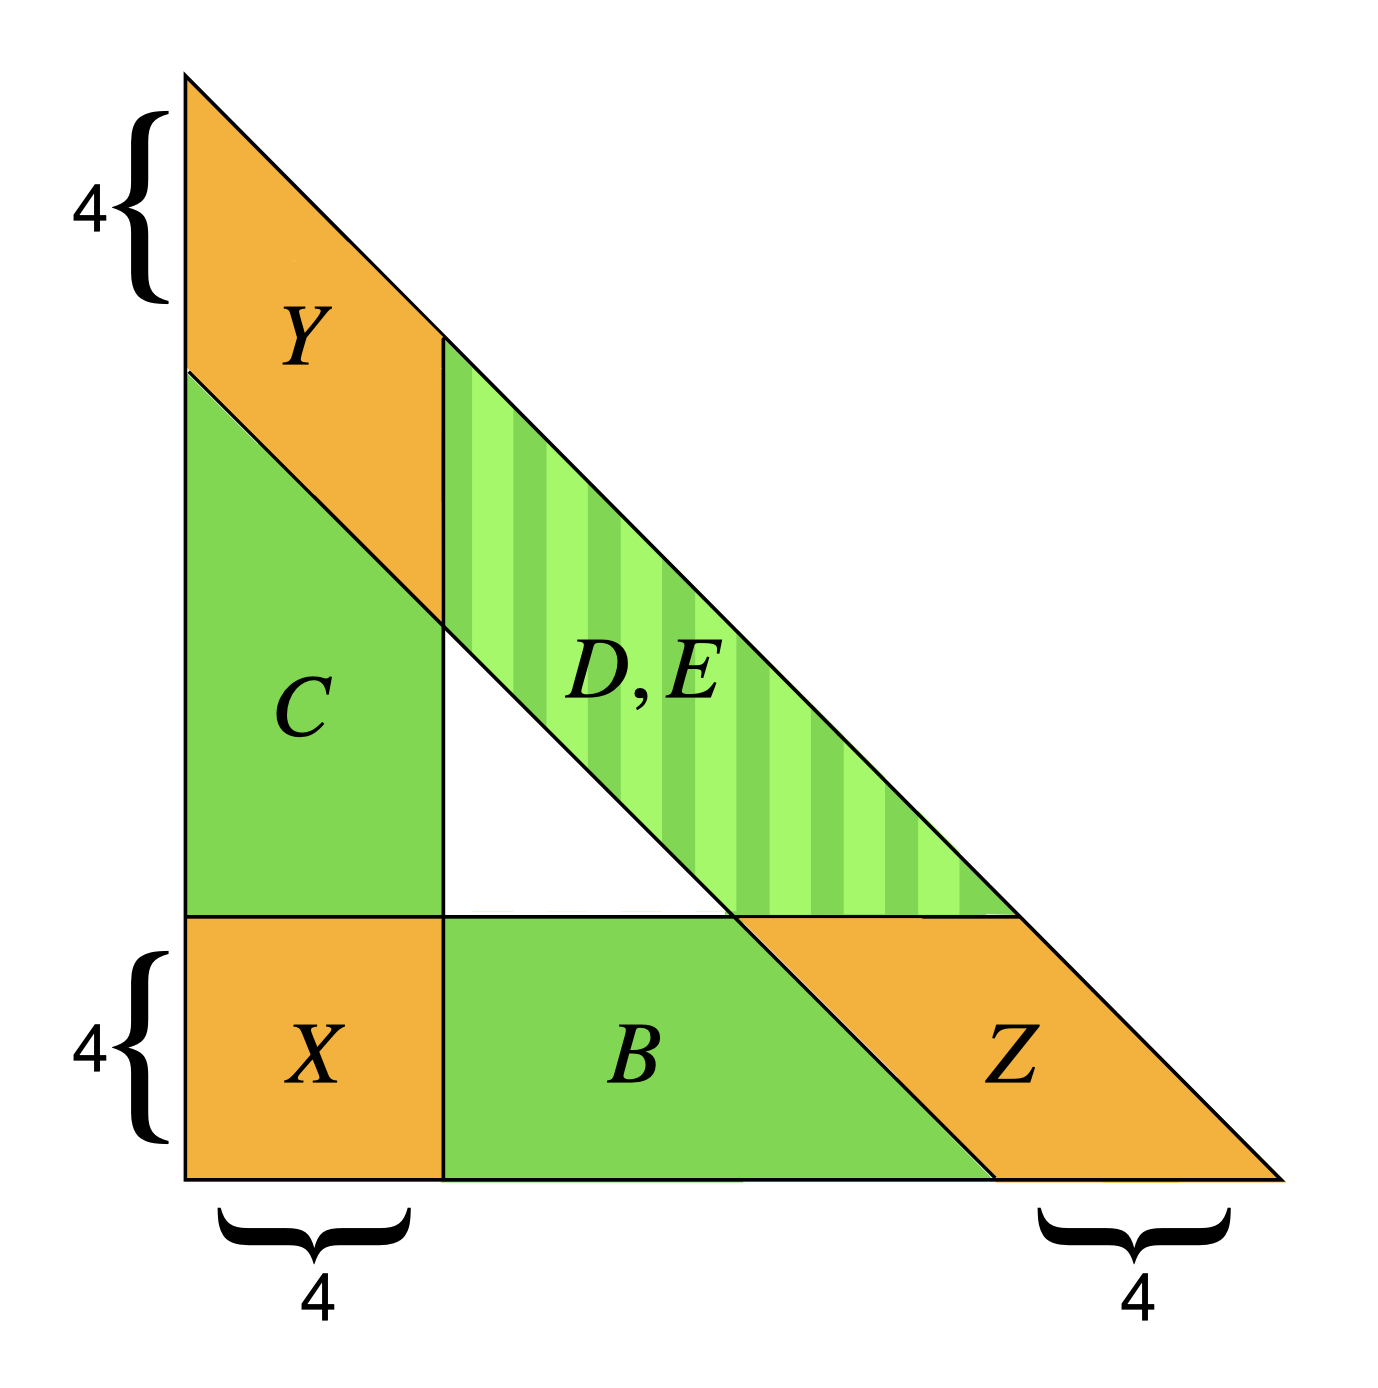
\includegraphics[width=0.8\textwidth]{assets/contactions-4.png}
    \caption{This figure illustrates the contraction variables. The yellow areas \( X, Y, Z \) represent formal variables \( x_{i,j} \) that remain unaffected by the contraction. Each green area \( B, C, D, E \) represents rows or columns of vertices that are merged into a single vertex.}\label{fig:contractions-42342432}
\end{figure}

\begin{definition}\label{def:contraction-variables}
Let \( x_{i,j} \) be formal variables indexed by \( V_d \). We merge a subset of rows and columns into a single vertex by defining \emph{contraction variables}:
\begin{align*}
    y_{i,j} &\coloneqq x_{i, d-3-i+j} \quad \text{ for } i,j = 0, \dots, 3, \\
    z_{i,j} &\coloneqq x_{d-3-j+i,j} \quad \text{ for } i,j = 0, \dots, 3, \\
    b_j &\coloneqq x_{4,j} + \dots + x_{d-4-j,j} \quad \text{ for } j = 0, \dots, 3, \\
    c_i &\coloneqq x_{i,4} + \dots + x_{i,d-4-i} \quad \text{ for } i = 0, \dots, 3, \\
    d_k &\coloneqq \begin{cases}
        x_{4,d-4-k} + x_{6,d-6-k} + \dots + x_{d-4-k,4} & \text{ if \( d + k \) is even} \\
        x_{4,d-4-k} + x_{6,d-6-k} + \dots + x_{d-5-k,5} & \text{ if \( d + k \) is odd}
    \end{cases} \quad \text{ for } k = 0, \dots, 3, \\
    e_k &\coloneqq \begin{cases}
        x_{5,d-5-k} + x_{7,d-7-k} + \dots + x_{d-5-k,5} & \text{ if \( d + k \) is even} \\
        x_{5,d-5-k} + x_{7,d-7-k} + \dots + x_{d-4-k,4} & \text{ if \( d + k \) is odd}
    \end{cases} \quad \text{ for } k = 0, \dots, 3.
\end{align*}
\end{definition}

Let us visualize the contraction variables for \( d = 16 \) in the following figure.

\begin{figure}[H]
    \begin{align*}
        \begin{array}{cccccccccccccccccccc}
            y_{0,3} & & & & & & & & & & & & \\
            y_{0,2} & y_{1,3} & & & & & & & & & & & \\
            y_{0,1} & y_{1,2} & y_{2,3} & & & & & & & & & & \\
            y_{0,0} & y_{1,1} & y_{2,2} & y_{3,3} & & & & & & & & & \\
            c_0 & y_{1,0} & y_{2,1} & y_{3,2} & d_0 & & & & & & & & \\
            c_0 & c_1 & y_{2,0} & y_{3,1} & d_1 & e_0 & & & & & & & \\
            c_0 & c_1 & c_2 & y_{3,0} & d_2 & e_1 & d_0 & & & & & & \\
            c_0 & c_1 & c_2 & c_3 & d_3 & e_2 & d_1 & e_0 & & & & & \\
            c_0 & c_1 & c_2 & c_3 &  *  & e_3 & d_2 & e_1 & d_0 & & & & \\
            c_0 & c_1 & c_2 & c_3 &  *  & * & d_3 & e_2 & d_1 & e_0 & & & \\
            c_0 & c_1 & c_2 & c_3 &  *  & * & * & e_3 & d_2 & e_1 & d_0 & & \\
            c_0 & c_1 & c_2 & c_3 &  *  & * & * & * & d_3 & e_2 & d_1 & e_0 & \\
            c_0 & c_1 & c_2 & c_3 &  *  & * & * & * & * & e_3 & d_2 & e_1 & d_0 \\
            x_{0,3} & x_{1,3} & x_{2,3} & x_{3,3} & b_3 & b_3 & b_3 & b_3 & b_3 & b_3 & z_{0,3} & z_{1,3} & z_{2,3} & z_{3,3} \\
            x_{0,2} & x_{1,2} & x_{2,2} & x_{3,2} & b_2 & b_2 & b_2 & b_2 & b_2 & b_2 & b_2 & z_{0,2} & z_{1,2} & z_{2,2} & z_{3,2} \\
            x_{0,1} & x_{1,1} & x_{2,1} & x_{3,1} & b_1 & b_1 & b_1 & b_1 & b_1 & b_1 & b_1 & b_1 & z_{0,1} & z_{1,1} & z_{2,1} & z_{3,1} \\
            x_{0,0} & x_{1,0} & x_{2,0} & x_{3,0} & b_0 & b_0 & b_0 & b_0 & b_0 & b_0 & b_0 & b_0 & b_0 & z_{0,0} & z_{1,0} & z_{2,0} & z_{3,0}
        \end{array}
    \end{align*}  
\end{figure}

As we can see, the vertices \( x_{0,4}, \dots, x_{0, d-4} \) are merged into the contraction variable \( c_0 \) by summing them up. The key insight is that some hyperfield Pascal forms \( \sum_{(i,j) \in V_d} \lambda_{i,j} x_{i,j} \) can be expressed in terms of contraction variables.

\pagebreak

\begin{example}
    Consider \( \mathrm{sign}(\mathrm{diag}(1)) \) in \( {H}^{V_{16}} \). It is depicted in the following figure:
    \begin{verbatim}
        .
        +  +
        +  +  . 
        +  +  .  .  
        +  +  .  .  .  
        +  +  .  .  .  .  
        +  +  .  .  .  .  .  
        +  +  .  .  .  .  .  .  
        +  +  .  .  .  .  .  .  .
        +  +  .  .  .  .  .  .  .  .  
        +  +  .  .  .  .  .  .  .  .  .
        +  +  .  .  .  .  .  .  .  .  .  .
        +  +  .  .  .  .  .  .  .  .  .  .  .
        +  +  .  .  .  .  .  .  .  .  .  .  .  .
        +  +  .  .  .  .  .  .  .  .  .  .  .  .  .
        +  +  .  .  .  .  .  .  .  .  .  .  .  .  .  .
        +  +  .  .  .  .  .  .  .  .  .  .  .  .  .  .  .
    \end{verbatim}
    We see that \( \mathrm{sign}(\mathrm{diag}(1)) = x_{0,0} + x_{0,1} + x_{0,2} + x_{0,3} + x_{1,0} + x_{1,1} + x_{1,2} + x_{1,3} + y_{0,0} + y_{0,1} + y_{0,2} + y_{1,0} + y_{1,1} + y_{1,2} + y_{1,3} + c_0 + c_1\). Note that this expression is \emph{independent} of the degree \( d \),
\end{example}

\begin{definition}
    Let \( d \in \mathbb{N}_{\geq 11} \) and \( p \) be a hyperfield linear form on \( H^{V_d} \). We say \( p \) is \emph{contractable} for \( d \) if we can write \( p = \hat p \) for some linear form \( \hat p \in H[\mathbf{x}, \mathbf{y}, \mathbf{z}, \mathbf{b}, \mathbf{c}, \mathbf{d}, \mathbf{e}] \). 
\end{definition}

\begin{definition}
    Let \( t \) be a formal variable. Define \( I = \left\{ 0,1,2,3,4,t-4,t-3,t-2,t-1,t \right\} \). Let \( T \) be a formal linear combination of
    \begin{align*}
        \left\{\mathrm{diag}(k), \mathrm{row}(k), \mathrm{col}(k) \right\}_{k \in I} \text{ or }\left\{\mathrm{sign}(\mathrm{diag}(k)), \mathrm{sign}(\mathrm{row}(k)), \mathrm{sign}(\mathrm{col}(k)) \right\}_{k \in I}.
    \end{align*}
    Let \( d \in \mathbb{N}_{\geq 11}\). We write \( p_d \) for the realization of \( T \) at \( t = d \); the realization \( p_d \) is just a linear form on \( \mathbb{Z}^{V_d} \) or  \( H^{V_d} \), respectively, where the formal variable \( t \) is replaced by the actual value \( d \).
\end{definition}


\begin{example}
    Let \( d = 15 \). Consider the formal linear combination \( T = \mathrm{row}(3) - \mathrm{row}(t - 2) \). The realization \( p_d \) of \( T \) at \( t = d \) is the linear form \( p = \mathrm{row}(3) - \mathrm{row}(13) \). It is depicted in the figure below. Note that the realization \( p_d \) is contractable for all \( d \in \mathbb{N} \) with \( d \geq 15 \). So, we ask whether the linear form \( \hat p_d \in H[\mathbf{x}, \mathbf{y}, \mathbf{z}, \mathbf{b}, \mathbf{c}, \mathbf{d}, \mathbf{e}]\) change with \( d \)? 

    \pagebreak
    \begin{verbatim}
-350 
-350   . 
-285  65  65 
-220  65   . -65 
-165  55 -10 -10  55 
-120  45 -10   .  10 -45 
 -84  36  -9   1   1  -9  36 
 -56  28  -8   1   .  -1   8 -28 
 -35  21  -7   1   .   .   1  -7  21 
 -20  15  -6   1   .   .   .  -1   6 -15 
 -10  10  -5   1   .   .   .   .   1  -5  10 
  -4   6  -4   1   .   .   .   .   .  -1   4  -6 
  -1   3  -3   1   .   .   .   .   .   .   1  -3   3 
   .   1  -2   1   .   .   .   .   .   .   .  -1   2  -1 
   .   .  -1   1   .   .   .   .   .   .   .   .   1  -1   . 
   .   .   .   1   .   .   .   .   .   .   .   .   .  -1   .   .         
    \end{verbatim}
    
\end{example}

\begin{definition}
    Let \( D \in \mathbb{N} \) and \( T \) be a formal linear combination of
    \begin{align*}
        \left\{ \mathrm{sign}(\mathrm{diag}(k)), \mathrm{sign}(\mathrm{row}(k)), \mathrm{sign}(\mathrm{col}(k)) \right\}_{k \in \left\{ 0,1,2,3,4,t-4,t-3,t-2,t-1,t \right\}}.
    \end{align*}
    We say \( T \) is \emph{fixed-contractable} starting from degree \( D \) if all the following statements hold:
    \begin{enumerate}
        \item The realization \( p_d \) is contractable for all \( d \geq D \);
        \item There exists a linear form \( \hat p^{\mathrm{even}} \in H[\mathbf{x}, \mathbf{y}, \mathbf{z}, \mathbf{b}, \mathbf{c}, \mathbf{d}, \mathbf{e}] \) such that \( p_d = \hat p^{\mathrm{even}} \) for all even degrees \(  d \geq D  \);
        \item There exists a linear form \( \hat p^{\mathrm{odd}} \in H[\mathbf{x}, \mathbf{y}, \mathbf{z}, \mathbf{b}, \mathbf{c}, \mathbf{d}, \mathbf{e}] \) such that \( p_d = \hat p^{\mathrm{odd}} \) for all odd degrees \( d \geq D  \).
    \end{enumerate}
\end{definition}


\begin{proposition}\label{prop:contracted-part-1}
    Let \( T \in \left\{ \mathrm{sign}(\mathrm{diag}(k)), \mathrm{sign}(\mathrm{row}(k)), \mathrm{sign}(\mathrm{col}(k)) \right\}_{k \in \left\{ 0,1,2,3,4,t-4,t-3,t-2,t-1,t \right\}}\) be a formal form. Then, \( T \) is fixed-contractable starting from degree \( D = 11 \).
\end{proposition}

\begin{proof}
    Let \( d \geq 11 \).
    We have the following cases:
    \begin{enumerate}
        \item Let \( T \in \left\{ \mathrm{sign}(\mathrm{row}(k)), \mathrm{sign}(\mathrm{diag}(k)) \mid k = 0,1,2,3 \right\} \). We observe that the hyperfield form \( p_d \) has support contained in the areas \( X, C \), and \( Y \) from Figure \ref{fig:contractions-42342432}. This follows directly from Proposition \ref{skdmldskfmksdej}. We also see that \( p_d \) depends only on the column sums on \( C \).
        \item Let \( T \in \left\{ \mathrm{sign}(\mathrm{col}(k)), \mathrm{sign}(\mathrm{diag}(t-k)) \mid k = 0,1,2,3 \right\} \). We see that \( p_d \) has support contained in the areas \( X, B \), and \( Z \) from Figure \ref{fig:contractions-42342432} by Proposition \ref{skdmldskfmksdej}. We conclude that \( p_d \) only depends on the row sums on \( B \).
        \item Let \( T \in \left\{ \mathrm{sign}(\mathrm{col}(t-k)), \mathrm{sign}(\mathrm{row}(t-k)) \mid k = 0,1,2,3 \right\} \). All the hyperfield forms \( p_d \) depend on entries in the area \( Y, D \), and \( Z \) from Figure \ref{fig:contractions-42342432} by Proposition \ref{skdmldskfmksdej}. We see that \( p_d \) depends in area \( D \) on alternating diagonal sums. This shows that \( p_d \) is a sum of the contraction variables \( y_{i,j} \), \( z_{i,j} \), and \( d_k - e_k \).

    \end{enumerate}
\end{proof}


\begin{example}
    The support of \( \mathrm{sign}(\mathrm{col}(d-3)) \) is depicted for \( d = 12 \) and \( d = 13 \):
    \begin{verbatim}
                             · 
·                            · ·    
· ·                          · · ·
· · ·                        + + + + 
+ + + +                      · - - - - 
· - - - -                    · · + + + + 
· · + + + +                  · · · - - - - 
· · · - - - -                · · · · + + + + 
· · · · + + + +              · · · · · - - - - 
· · · · · - - - -            · · · · · · + + + + 
· · · · · · + + + +          · · · · · · · - - - - 
· · · · · · · - - - -        · · · · · · · · + + + + 
· · · · · · · · + + + +      · · · · · · · · · - - - -
· · · · · · · · · - - - -    · · · · · · · · · · + + + +
    \end{verbatim}
    For \( d = 12 \), we write \( \mathrm{sign}(\mathrm{col}(d-3)) = \sum^3_{i=0}\sum^i_{j=0} (-1)^{i+j}y_{i,j} - \sum^3_{k=0}(-1)^{k}d_k  + \sum^3_{k=0}(-1)^{k}e_k - \sum^3_{i,j=0}(-1)^{j}z_{i,j} \). For \( d = 13 \) we write \( \mathrm{sign}(\mathrm{col}(d-3)) = \sum^3_{i=0}\sum^i_{j=0} (-1)^{i+j}y_{i,j} - \sum^3_{k=0}(-1)^{k}d_k  + \sum^3_{k=0}(-1)^{k}e_k + \sum^3_{i,j=0}(-1)^{j}z_{i,j} \).
\end{example}

We have merged formal variables \( x_{i,j} \) indexed by vertices \( (i,j) \) in the areas \( B, C, D \) into contraction variables. We also see that our row, column, and diagonal Pascal forms can be expressed by contraction variables; even more, this contraction form is independent of the degree \( d \). Let us apply these contractions to concrete elements \( \mathbf{s} \in H^{V_d} \).

\begin{definition}
    We define the index set \(  \Xi \coloneqq \left\{ 0,1,2,3 \right\}^2 \sqcup \left\{ 0,1,2,3 \right\}^2 \sqcup \left\{ 0,1,2,3 \right\}^2 \sqcup \left\{ 0,1,2,3 \right\} \sqcup \left\{ 0,1,2,3 \right\} \sqcup \left\{ 0,1,2,3 \right\} \sqcup \left\{ 0,1,2,3 \right\} \).
    Let \( \mathbf{s} \in H^{\Xi} \). We call \( \mathbf{s} \) a \emph{contracted hyperfield configuration}, and write \( \mathbf{s} = (\mathbf{x}, \mathbf{y}, \mathbf{z}, \mathbf{b}, \mathbf{c}, \mathbf{d}, \mathbf{e}) = (x_{i,j}, y_{i,j}, z_{i,j}, b_j, c_i, d_k, e_k) \).
\end{definition}

\begin{definition}
    Let \( \mathbf{s} \in H^{\Xi}\) be a {contracted hyperfield configuration}.
    We say \( \mathbf{s} \) is \emph{valid} if one of the following holds:
    \begin{enumerate}
        \item \( \mathbf{s} = \mathbf{0} \) or
        \item \( s_{0,0} = -1 \), \( x_{i,j} \geq 0 \) for all \( i+j > 0 \), and \(  y_{i,j}, z_{i,j}, b_j, c_i, d_k, e_k \geq 0 \) for all \( i,j,k = 0,1,2,3 \).
    \end{enumerate}
\end{definition}

Going from the world of hyperfield configurations to the world of \emph{contracted} hyperfield configurations is achieved via the following map.

\begin{definition}
    Let \( d \geq 11 \). Let \( \mathbf{s} \in H^{V_d} \) be a hyperfield configuration. We define 
    \begin{align*}
        \mathrm{contr}_d(\mathbf{s}): \mathbf{s} \mapsto (\mathbf{x}, \mathbf{y}, \mathbf{z}, \mathbf{b}, \mathbf{c}, \mathbf{d}, \mathbf{e}) = (x_{i,j}, y_{i,j}, z_{i,j}, b_j, c_i, d_k, e_k)
    \end{align*}
    where we set
    \begin{align*}
        x_{i,j} &\coloneqq s_{i,j} \quad \text{ for } i,j = 0, \dots, 3, \\
        y_{i,j} &\coloneqq s_{i, d-3-i+j} \quad \text{ for } i,j = 0, \dots, 3, \\
        z_{i,j} &\coloneqq s_{d-3-j+i,j} \quad \text{ for } i,j = 0, \dots, 3, \\
        b_j &\coloneqq s_{4,j} + \dots + s_{d-4-j,j} \quad \text{ for } j = 0, \dots, 3, \\
        c_i &\coloneqq s_{i,4} + \dots + s_{i,d-4-i} \quad \text{ for } i = 0, \dots, 3, \\
        d_k &\coloneqq \begin{cases}
            s_{4,d-4-k} + s_{6,d-6-k} + \dots + s_{d-4-k,4} & \text{ if \( d + k \) is even} \\
            s_{4,d-4-k} + s_{6,d-6-k} + \dots + s_{d-5-k,5} & \text{ if \( d + k \) is odd}
        \end{cases} \quad \text{ for } k = 0, \dots, 3, \\
        e_k &\coloneqq \begin{cases}
            s_{5,d-5-k} + s_{7,d-7-k} + \dots + s_{d-5-k,5} & \text{ if \( d + k \) is even} \\
            s_{5,d-5-k} + s_{7,d-7-k} + \dots + s_{d-4-k,4} & \text{ if \( d + k \) is odd}
        \end{cases} \quad \text{ for } k = 0, \dots, 3.
    \end{align*}
\end{definition}

The contraction map \( \mathrm{contr}_d \) maps hyperfield configurations \( \mathbf{s} = (\mathbf{x}, \mathbf{y}, \mathbf{z}, \mathbf{b}, \mathbf{c}, \mathbf{d}, \mathbf{e}) \in H^{{V_d}} \) to elements in \( H^{\Xi} \) if \( \mathbf{b}, \mathbf{c}, \mathbf{d}, \mathbf{e}  \geq 0\). If one of the entries is negative, the map may output to some element \( (2^H)^{\Xi} \). To make life easier, we only consider \emph{weakly valid} configuration; these are configurations whose negative support is only contained in the yellow area below.

\begin{figure}[H]
    \centering
    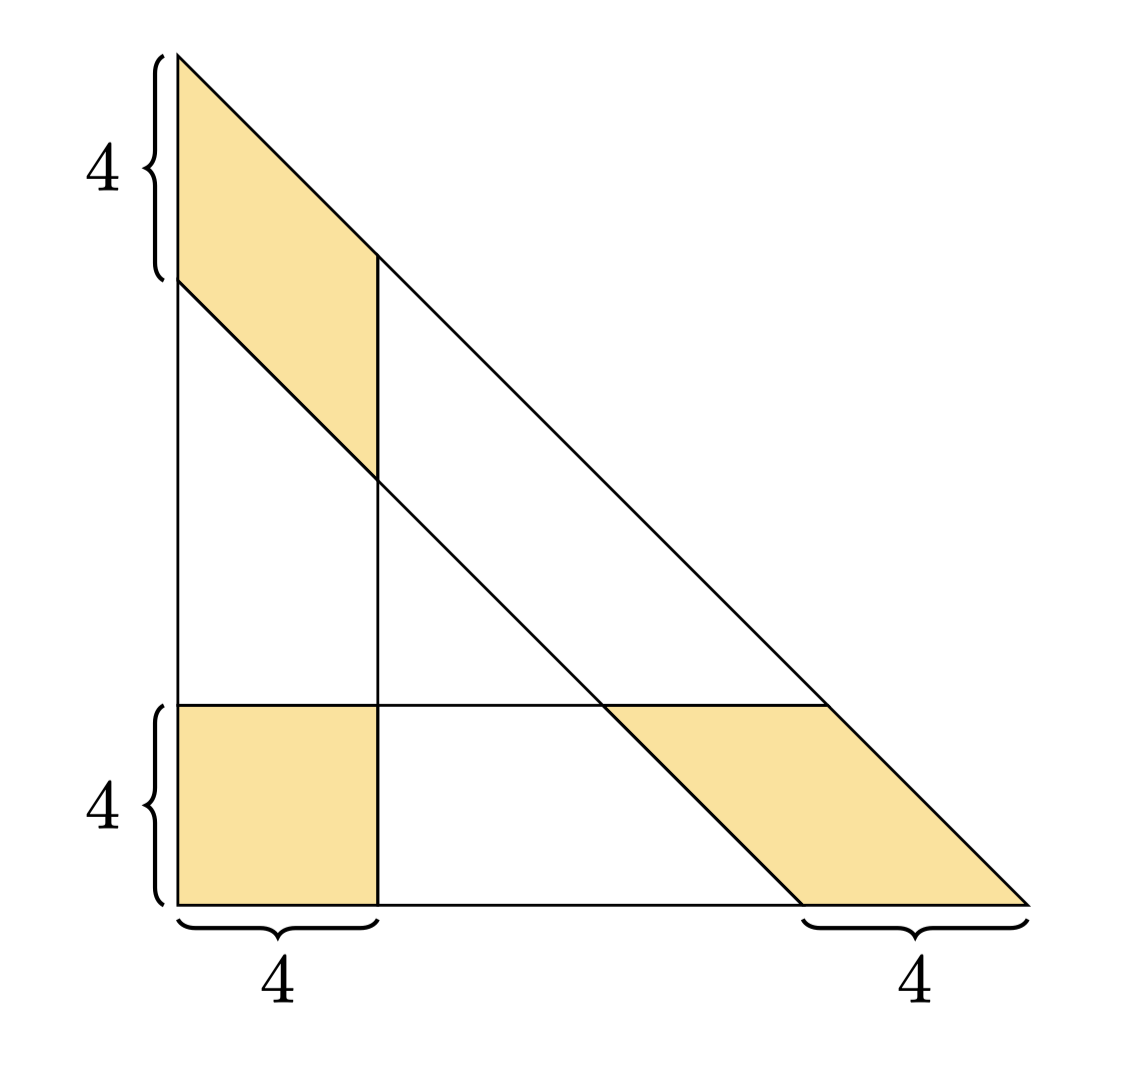
\includegraphics[width=0.4\textwidth]{assets/weakly-valid.png}
    \caption{A hyperfield configuration is weakly valid if its negative support is contained in the yellow area.}
\end{figure}

\begin{definition}
    Let \( \mathbf{s} \in H^{V_d} \) be a hyperfield configuration. We say \( \mathbf{s} \) is \emph{weakly valid} if for all \( (i,j) \in \mathrm{supp}^-(\mathbf{s}) \) one of the following holds:
    \begin{enumerate}
        \item \( i,j = 0, \dots, 3 \), or
        \item \( i = 0, \dots, 3 \) and \( i+j \geq d-3 \), or
        \item \( j = 0, \dots, 3 \) and \( i + j \geq d-3 \).
    \end{enumerate}
\end{definition}

\begin{definition}
    Let \( \mathbf{s} \in H^{\Xi} \) be a contracted hyperfield configuration. The \emph{positive support} of \( \mathbf{s} = (\mathbf{x}, \mathbf{y}, \mathbf{z}, \mathbf{b}, \mathbf{c}, \mathbf{d}, \mathbf{e}) \) is defined as the set of all symbols \( x_{i,j}, y_{i,j}, z_{i,j}, b_j, c_i, d_k, e_k \) such that the corresponding coefficients of \( \mathbf{s} \) equal to one.
\end{definition}

\begin{example}
    Let \( \mathbf{s} = (\mathbf{x}, \mathbf{y}, \mathbf{z}, \mathbf{b}, \mathbf{c}, \mathbf{d}, \mathbf{e}) \in H^{\Xi}\) be a contracted hyperfield configuration defined by \( x_{0,0} = -1,  x_{0,3} = 1,  x_{1,1} = 1, x_{3,0} = 1, d_0 = 1,  e_0 = 1 \), and all other entries are zero. Then, the positive support of \( \mathbf{s} \) is given by \( \mathrm{supp}^+(\mathbf{s}) = \left\{ x_{0,3}, x_{1,1}, x_{3,0}, d_0, e_0 \right\} \).
\end{example}

\section{Proof}

We now prove that for every valid outcome \( \mathbf{w} \) with \( |\mathrm{supp}^+(\mathbf{w})| = 4 \), we have \( \mathrm{deg}(\mathbf{w}) \leq 5 \). Define two systems of Pascal forms that valid outcomes must satisfy: 
\begin{enumerate}
    \item \( \Phi_1 \coloneqq \left\{ \mathrm{col}(i), \mathrm{row}(i), \mathrm{diag}(i), \mathrm{diag}(d-i) \right\}_{i=1}^3 \), 
    \item \( \Phi_2 \coloneqq \left\{ \mathrm{row}(d-i), \mathrm{col}(d-i) \right\}_{i=0}^3 \), and 
    \item \( \Phi \coloneqq \Phi_1 \cup \Phi_2 \).
\end{enumerate}



By Proposition \ref{prop:contracted-part-1}, we write all forms \( p \) in \( \Phi_1 \) as \( \mathrm{sign}(p) = \hat p \)
for some linear form \( \hat p \in H[\mathbf{x}, \mathbf{y}, \mathbf{z}, \mathbf{b}, \mathbf{c}, \mathbf{d}, \mathbf{e}] \) if \( d \geq 11 \). This linear form is independent of the degree \( d \). To make notations consistent later, we set \( \hat p^{\mathrm{even}} \coloneqq  \hat p^{\mathrm{odd}}  \coloneqq \hat p\). Similarly, by Proposition \ref{prop:contracted-part-1}, we write all forms \( p \) in \( \Phi_2 \) as \( \mathrm{sign}(p) = \begin{cases}
    \hat p^{\mathrm{even}} & \text{ if } d \text{ is even} \\
    \hat p^{\mathrm{odd}} & \text{ if } d \text{ is odd}
\end{cases} \), where \( \hat p^{\mathrm{even}}, \hat p^{\mathrm{odd}} \in H[\mathbf{x}, \mathbf{y}, \mathbf{z}, \mathbf{b}, \mathbf{c}, \mathbf{d}, \mathbf{e}] \) if \( d \geq 12 \). Again, these linear forms \( \hat p^{\mathrm{even}}, \hat p^{\mathrm{odd}}  \) are independent of the degree \( d \).

\begin{definition}\label{def:sdjsndjknsdj}
    We define the following three solution sets:
    \begin{enumerate}
        \item     Define \( \Gamma_d \) to be the set of all valid hyperfield configurations \( \mathbf{s} \in H^{V_d} \) of degree \( d \) such that \( \mathrm{sign}(p)(\mathbf{s}) = H \) for all \( p \in \Phi \).

        \item     Define \( \Gamma^{\mathrm{even}} \) to be the set of all valid contracted hyperfield configurations \( \mathbf{s} \in H^{\Xi} \) such that \( \hat p^{\mathrm{even}}(\mathbf{s}) = H \) for all \( p \in \Phi \).

        \item     Define \( \Gamma^{\mathrm{odd}} \) to be the set of all valid contracted hyperfield configurations \( \mathbf{s} \in H^{\Xi} \) such that \( \hat p^{\mathrm{odd}}(\mathbf{s}) = H \) for all \( p \in \Phi \).
    \end{enumerate}
\end{definition}

By Proposition \ref{prop:hyperfield-criterion}, valid chipsplitting outcomes of degree \( d \) have supports in \( \Gamma_d \). 

\begin{proposition}\label{prop:sign-sikjsfnf3223423432}
    Let \( d \geq 12 \). If \( d \) is even, then \( \Gamma_d = \mathrm{contr}_d^{-1}(\Gamma^{\mathrm{even}}) \) holds. If \( d \) is odd, then \( \Gamma_d = \mathrm{contr}_d^{-1}(\Gamma^{\mathrm{odd}}) \) holds.
\end{proposition}

\begin{proof}
    Let \( d \geq 12 \) be even. Let \( \mathbf{s} \in {H}^{V_d} \) be a hyperfield configuration and \( p \in \Phi \). Then, we have \( \mathrm{sign}(p)(\mathbf{s}) = \hat p^{\mathrm{even}}(\mathrm{contr}_d(\mathbf{s})) \)
    by definition of \( \hat p^{\mathrm{even}} \). If \( \mathbf{s} \in \Gamma_d \), then \( H = \mathrm{sign}(p)(\mathbf{s}) = \hat p^{\mathrm{even}}(\mathrm{contr}_d(\mathbf{s})) \). Hence, \( \mathrm{contr}_d(\mathbf{s}) \) is contained in \( \Gamma^{\mathrm{even}} \). If \( \mathrm{contr}_d(\mathbf{s}) \in \Gamma^{\mathrm{even}} \) holds, using the equation above we also see that \( \mathbf{s} \in \Gamma_d \). This shows that \( \Gamma_d = \mathrm{contr}_d^{-1}(\Gamma^{\mathrm{even}}) \).

    The second statement for odd degrees \( d \) follows analogously.
\end{proof}

\begin{corollary}\label{cor:validwunfwufneuiw}
    Let \( d \geq 12 \) and \( \mathbf{w} \in \mathbb{Z}^{V_d} \) be a valid outcome. Then, we have \( \mathrm{contr}_d(\mathrm{sign}(\mathbf{w})) \in \Gamma^{\mathrm{even}} \cup \Gamma^{\mathrm{odd}} \).
\end{corollary}

\begin{proof}
    Define \( \mathbf{s} \coloneqq \mathrm{sign}(\mathbf{w}) \). By Proposition \ref{prop:sign-sikjsfnf322} we have \( \mathbf{s} \in \Gamma_d \). If \( d \) is even, then \( \mathrm{contr}_d(\mathbf{s}) \in \Gamma^{\mathrm{even}} \) by the previous proposition. If \( d \) is odd, then \( \mathrm{contr}_d(\mathbf{s}) \in \Gamma^{\mathrm{odd}} \) by the previous proposition.
\end{proof}

This corollary allows us to exclude certain supports as supports of valid outcomes. Assume we have a contracted hyperfield configuration \( \xi \in H^{\Xi} \) that is not a root of some \( \hat p \) for \( p \in \Phi \). Then, any chipsplitting configuration \( \mathbf{w} \in \mathbb{Z}^{V_d} \) with \( \mathrm{contr}_d( \mathrm{sign}(\mathbf{w})) = \xi \) is not a valid outcome.

\begin{proposition}\label{prop:jasndkjsnjsnkjs}
    Let \( \mathbf{s} \in H^{V_d} \) be a valid hyperfield configuration of degree \( d \) with positive support size four or less. If \( d\geq 12 \), then \( \mathbf{s} \notin \Gamma_d \).
\end{proposition}

\begin{proof}
    Let \( d \geq 12 \). For computing \( \Gamma_d \) we could use Algorithm \ref{alg:hyperfield_criterion:efficient} for all \( d = 12, 13, 14, \dots \) and so on, which is not feasible since we would compute solutions sets for many infinitely many degrees \( d \). Instead, we show that \( \Gamma^{\mathrm{even}} \cup \Gamma^{\mathrm{odd}} \) is empty. By Proposition \ref{prop:sign-sikjsfnf3223423432}, \( \Gamma_d \) is empty as well for all \( d\geq 12 \).

    To show that \(  \Gamma^{\mathrm{even}} \) is empty, we use Algorithm \ref{alg:hyperfield_criterion:efficient} and Remark \ref{rem:fiuhwiu3} with \(A \coloneqq \left\{ \hat p^{\mathrm{even}} \mid p \in \Phi \right\}\). Similarly, to compute that \( \Gamma^{\mathrm{odd}} \) is empty, we define \(A \coloneqq \left\{ \hat p^{\mathrm{odd}} \mid p \in \Phi \right\}\) and use Algorithm \ref{alg:hyperfield_criterion:efficient}. The implementation details are publicly available on GitHub in the file \texttt{chapter05.ipynb} \cite{ducrepo}.
\end{proof}

\begin{theorem}\label{thm:main-result-32432432432nkdnjkfd}
    For valid integral outcomes \( \mathbf w \) with \( |\mathrm{supp}^+(\mathbf w)| = 4 \) we have \( \mathrm{deg}(\mathbf w) \leq 5 \).
\end{theorem}

\begin{proof}
    Let \( d \geq 6 \).
    Let \( \mathbf{w} \in \mathbb{Z}^{V_d} \) be a valid outcome with \( |\mathrm{supp}^+(\mathbf w)| = 4 \) and degree \( d \). We have \( \mathrm{sign}(\mathbf{w}) \in \Gamma_d \). By the previous proposition, there is no such \( \mathrm{sign}(\mathbf{w}) \) for \( d \geq 12 \). By Proposition \ref{prop:jdngkjrenj3nw}, the degree of \( \mathrm{sign}(\mathbf{w}) = d \) is six or seven. So, we check eight cases. Of these eight cases, we exclude all of them by applying Algorithm \ref{alg:hyperfield_criterion:is_zero}, see the file \texttt{chapter05.ipynb} in \cite{ducrepo}.
\end{proof}